\documentclass[twoside,11pt]{article}

% Any additional packages needed should be included after obs_study_style.
% Note that obs_study_style.sty includes epsfig, amssymb, natbib and graphicx,
% and defines many common macros, such as 'proof' and 'example'.
%
% It also sets the bibliographystyle to plainnat; for more information on
% natbib citation styles, see the natbib documentation, a copy of which

\usepackage{obs_study_style}

\usepackage{tkz-graph}
\usetikzlibrary{shapes.geometric}
\usepackage{amsmath}
\usepackage{bbm}
\usepackage[hidelinks]{hyperref}
\usepackage{float}
\usepackage{graphicx}
\usepackage{caption}
\usepackage{subcaption}

% Definitions of handy macros can go here

\newtheorem{assumption}{Assumption}

\newcommand{\phuc}[1]{{\color{teal} {#1}}}
\newcommand{\todo}[1]{{\color{purple} todo: {#1}}}

% For papers submitted for review, just fill in author names
% For accepted papers, heading arguments are {volume}{year}{pages}{submitted}{published}{author-full-names}
\heading{}{}{}{}{}{Phuc Nguyen, David A. Pritchard, and Alan Brookhart}

% Short headings should be running head and authors last names

\ShortHeadings{The Accuracy of Psychohistorical Equations for Predicting the Results of Observational Studies}{Nguyen, Pritchard, and Brookhart}
\firstpageno{1}

\begin{document}

\title{Psychohistorical Equations for Observational Studies}

\author{\name Phuc Nguyen \email hseldon@streeling.edu \\
       \addr Department of Psychohistory\\
       Streeling University\\
       Trantor, Center of the Galaxy 94830, Galactic Empire 
       \AND
       \name David A. Pritchard \email david.al.pritchard@gmail.com \\
       \addr Department of Physics\\
       Pacific Tech \\
       Los Angeles, CA 90001, USA
       \AND
       \name Alan Brookhart \email mtaylor@pacifictech.edu \\
       \addr Department of Physics\\
       Pacific Tech \\
       Los Angeles, CA 90001, USA
       }

\maketitle

\begin{abstract}%   <- trailing '%' for backward compatibility of .sty file
\todo{}Psychohistory combines history, sociology, and mathematical statistics to make general predictions about the future behavior of very large groups of people. There are two axioms of psychohistory: (1) the population whose behaviour is modeled should be sufficiently large; (2) the population should remain in ignorance of the results of the application of psychohistorical analyses.  In this paper, we use psychohistory to predict the results of large observational studies.
\end{abstract}

\begin{keywords}
  \todo{}Mass Action, Prime Radiant, Survival Analysis
\end{keywords}

\section{Introduction}
\label{sec:introduction}

\subsection{Unmeasured confounding}

Under the potential outcome framework, a dichotomous counterfactual outcome variable $Y^a$ is the random variable that would have been observed under treatment $a$. For the common setting of a dichotomous treatment $A$, each individual has two potential outcomes $Y^{0}$, the outcome variable that would have been observed under the control treatment, and $Y^{1}$, the outcome variable that would have been observed under the experimental treatment \cite{hernan2010causal}. The average treatment effect (ATE) of a given treatment in a particular population is a widely-used causal estimand. For a dichotomous treatment, on the risk difference scale, the measure of the ATE in the population is defined as $E[Y^{1}] - E[Y^{0}]$. Similarly, the measure of the ATE on the risk ratio scale is defined as $E[Y^{1}] / E[Y^{0}]$. The measure of the average treatment effect on the treated (ATT), defined as $E[Y^{1}|A=1] - E[Y^{0}|A=1]$, is another estimand of interest.

In observational studies, the ATE can be identified---expressed as a function of the observed data---under identifying assumptions including consistency, no interference, positivity, and exchangeability \cite{naimi2023defining}. In this chapter, we focus solely on issues related to exchangeability being violated and hereafter assume consistency, no interference, and positivity hold. (Interested readers can see \cite{hernan2010causal, naimi2023defining} for details on the other assumptions.) Exchangeability means that the risk of the outcome under potential treatment $a$ is the same among the treated and untreated individuals, or $E[Y^a|A=0] = E[Y^a|A=1] \quad \forall a \in \{0, 1\}$:

\begin{assumption} (Exchangeability) \label{as:exchangeability}
  $Y^a \perp A \text{ for all } a$
\end{assumption}

Under exchangeability, the ATE is equivalent to the observed association,  e.g. the causal risk difference is equivalent to $E[Y | A = 1] - E[Y | A = 0]$. A weaker assumption known as conditional exchangeability also enables the identification of the ATE:

\begin{assumption} (Conditional exchangeability) \label{as:conditional-exchangeability}
  $Y^{a} \perp A | L \text{ for all } a$
\end{assumption}

\noindent where $L$ is a set of covariates. Under conditional exchangeability, the causal risk difference is:

\begin{equation}
E[Y^{1}] - E[Y^{0}] = \sum_{l} \Bigl( E[Y | A = 1, L = l] - E[Y | A = 0, L = l] \Bigr) P(L = l)
\end{equation}

Ideal randomized experiments automatically lead to exchangeability, however, observational studies often do not because factors $L$ used to determine treatment assignments are also likely to be associated with the outcome. The association between treatment $A$ and outcome $Y$ is then made up of the true causal effect and a bias induced by factors $L$. When factors $L$ are common causes of the treatment and the outcome, we refer to the bias as confounding \cite{hernan2010causal}. In observational studies of medical interventions, confounding is common as physicians prescribe treatments based on their assessment of a patient’s disease risk and patients seek treatment for reasons often related to prognosis \cite{brookhart2010confounding}. Under mild technical assumptions, confounding implies that exchangeability does not hold \cite{hernan2010causal}. However, conditional exchangeability can still hold if we have measured a sufficient set for confounding adjustment \cite{hernan2010causal}. We can determine this set using the backdoor criterion \cite{pearl1995causal} and the knowledge of the true causal directed acyclic graph (DAG) that generated the data. (See Chapter 7 in \cite{hernan2010causal} for more details.)

In practice, we can never guarantee that we have adjusted for a sufficient set, for instance, because we don't know the true causal DAG or because it's impossible to collect data on some variables.
Returning then to our previous example of healthcare studies where physicians prescribe the treatments of interest, it is likely impossible to be sure that the set of covariates being controlled for accounts for all possible risk factors for the outcome that influenced the treatment decision. Confounding that requires adjustment for unmeasured variables, which is impossible, is referred to as unmeasured confounding. Under mild technical assumptions, unmeasured confounding implies that conditional exchangeability also does not hold \cite{hernan2010causal}. It creates a systemic bias in the causal estimate that persists even as the study's sample size increases.
It is because of this clear opportunity for violation of identifying assumptions that unmeasured confounding is often considered to be the main threat to the validity of observational studies \cite{fewell2007impact}.
Although the no unmeasured confounding assumption is untestable \cite{shi2020selective}, negative controls are useful tools to detect and sometimes correct bias from unmeasured confounding \cite{lipsitch2010negative}.

\subsection{Negative controls}

Suppose that, in addition to measured variables $L$, there exist unmeasured common causes $U$ of the treatment $A$ and outcome $Y$. Given unmeasured confounders $U$, we have conditional exchangeability, that is $Y^a \perp A | U, L$ for all $a$. Let $N$ be a secondary outcome variable and $N^a$ be its potential outcome variable under treatment $a$. Outcome variable $N$ is a negative control outcome (NCO) if it satisfies the following \cite{shi2020selective}:

\begin{assumption} (Negative control outcome) \label{as:nco}
  $N^a = N \text{ and } N \perp A | U, L$ for all $a$
\end{assumption}

\begin{figure}[ht]
    \centering
    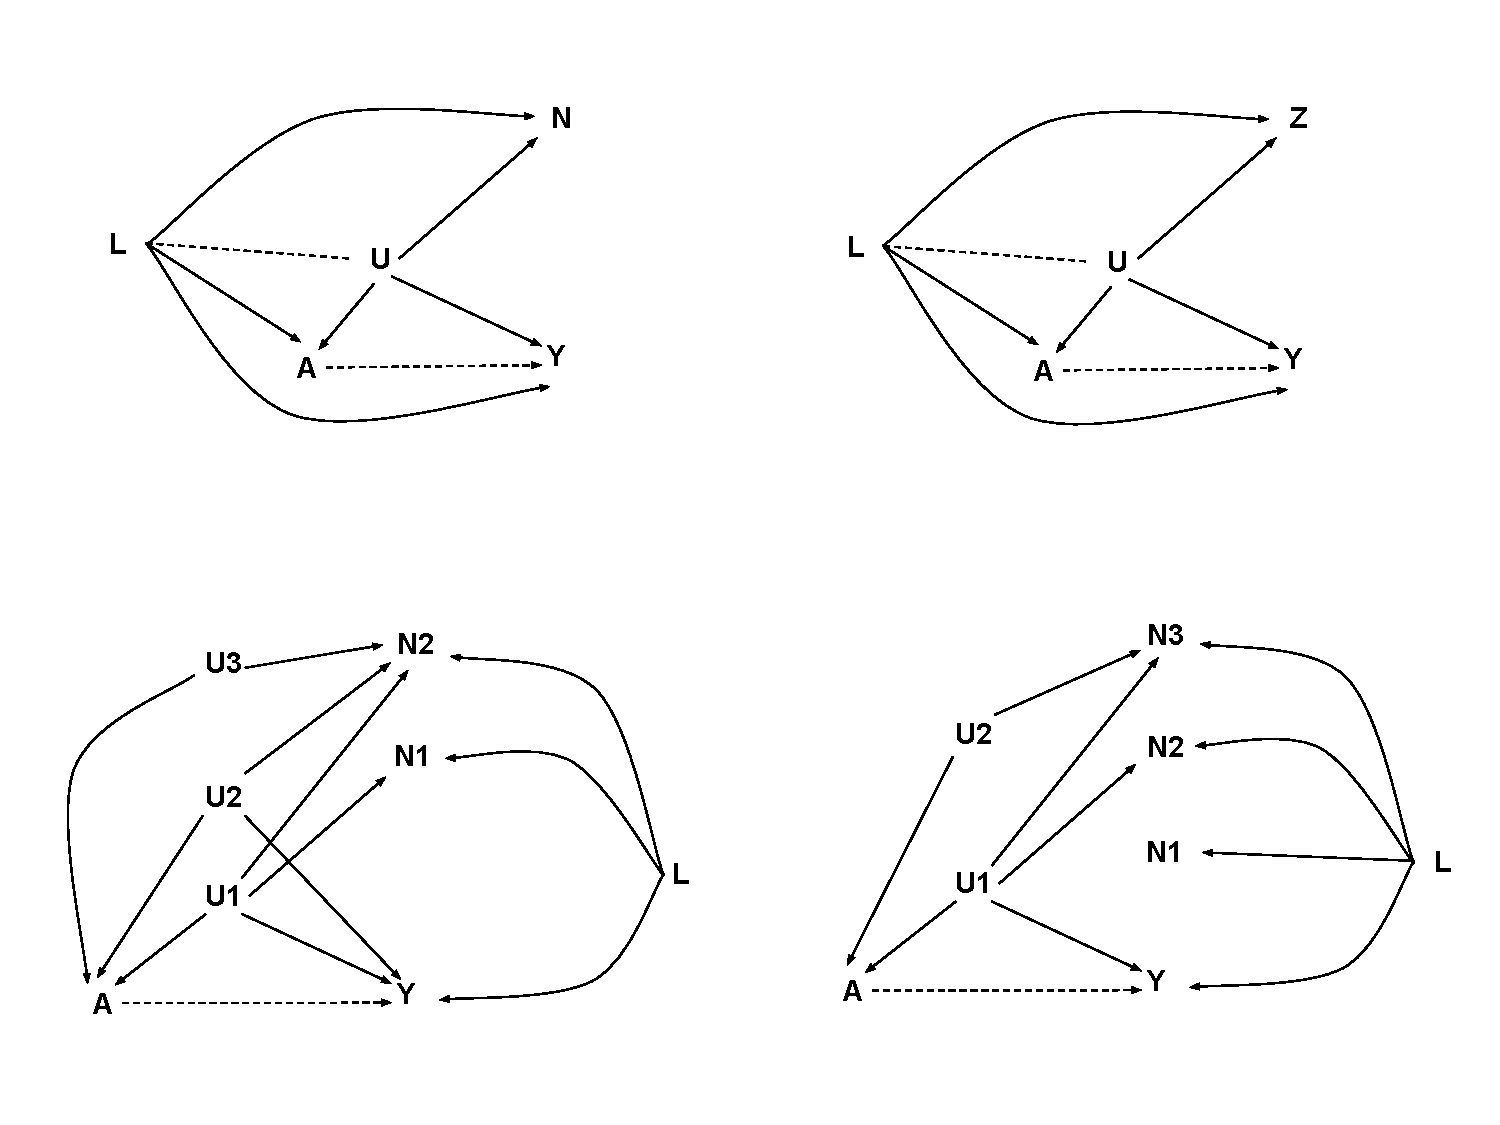
\includegraphics[trim={0 11cm 13cm 1.5cm}, clip, width=0.6\textwidth]{figures/dags.pdf}
    \caption[Causal DAG of an ideal NCO $N$ for bias detection/correction of the effect of treatment $A$ on outcome $Y$.]{Causal DAG of an ideal NCO $N$ for bias detection/correction of the effect of treatment $A$ on outcome $Y$, with observed confounders $L$ and unmeasured confounders $U$. Ideal NCOs have the same incoming arrows as $Y$, except that from $A$, and are U-comparable to $Y$ \cite{lipsitch2010negative}. A dashed line means that a relationship may exist.}
    \label{fig:nco-nco-dag}
\end{figure}

A secondary exposure $Z$ is a negative control exposure (NCE) if it satisfies the following \cite{shi2020selective}:

\begin{assumption} (Negative control exposure) \label{as:nce}
  $Y^{a,z} = Y^a \text{ and } Y^a \perp Z | U, L$ for all $a, z$
\end{assumption}

\begin{figure}[H]
    \centering
    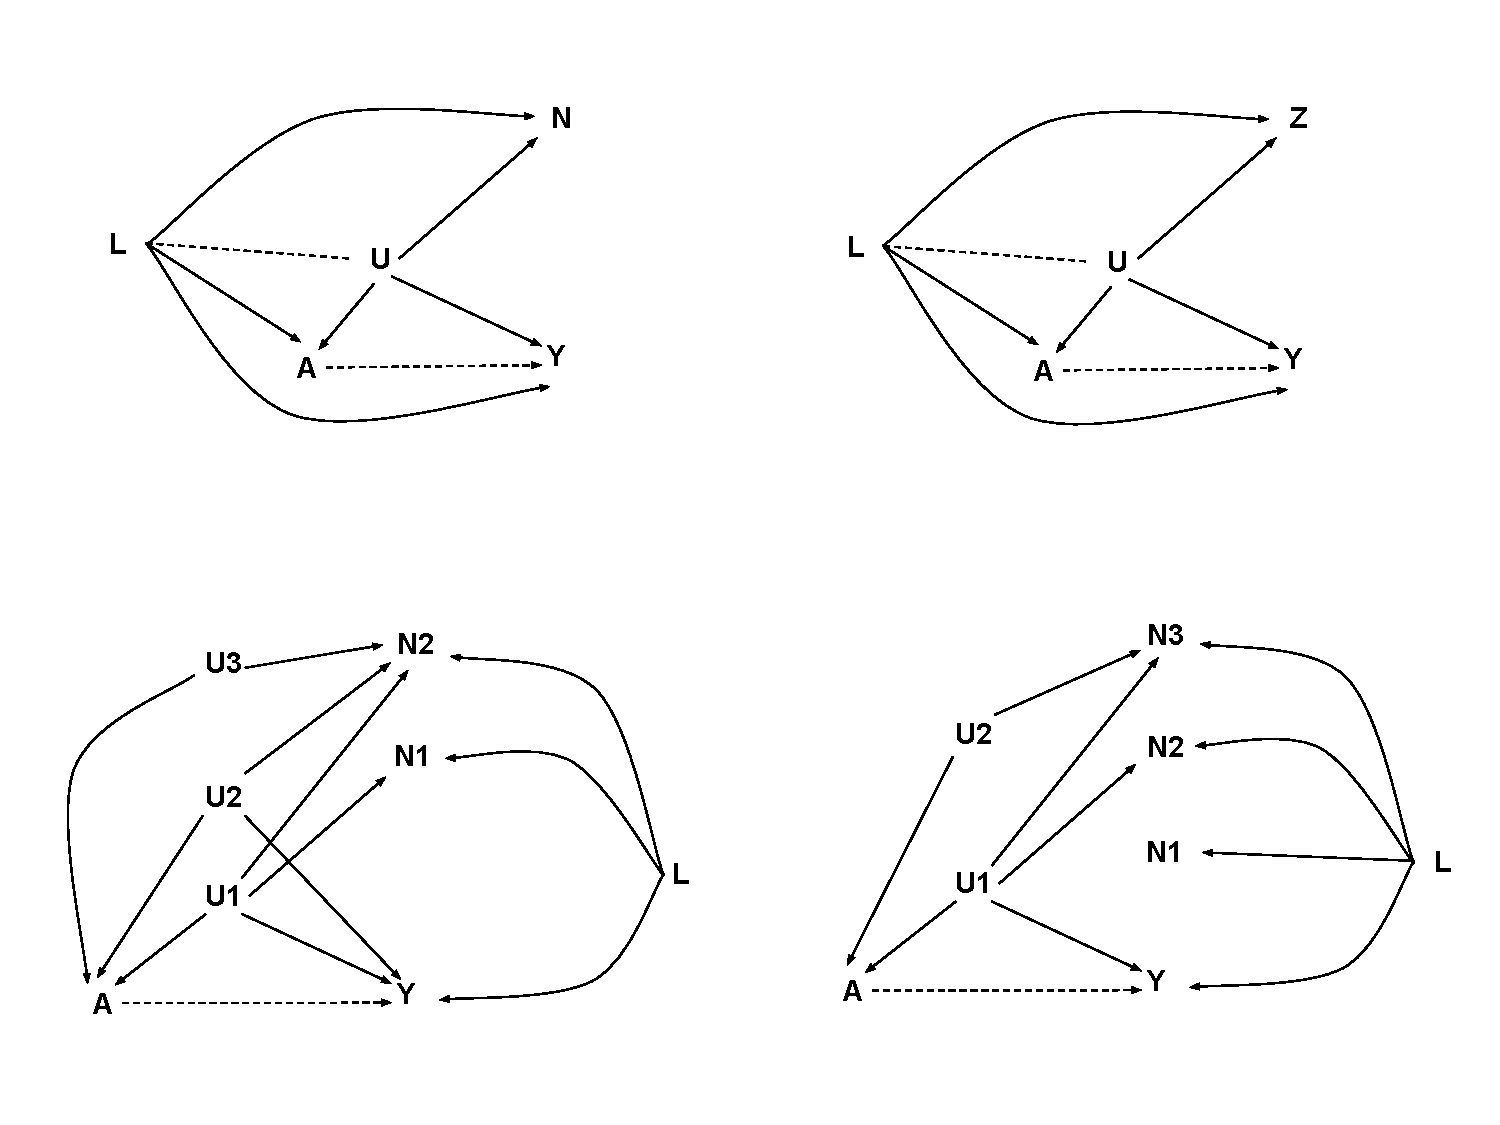
\includegraphics[trim={13cm 11cm 0 1.5cm}, clip, width=0.6\textwidth]{figures/dags.pdf}
    \caption[Causal DAG of an ideal NCE $Z$ for bias detection/correction of the effect of treatment $A$ on outcome $Y$.]{Causal DAG of an ideal NCE $Z$ for bias detection/correction of the effect of treatment $A$ on outcome $Y$, with observed confounders $L$ and unmeasured confounders $U$. Ideal NCEs have the same incoming arrows as $A$, and are U-comparable to $A$ \cite{lipsitch2010negative}.}
    \label{fig:nco-nce-dag}
\end{figure}

\noindent where $Y^{a, z}$ is the potential outcome variable under primary exposure $a$ and secondary exposure $z$. Informally, an NCO is a variable that is not causally affected by the treatment, and an NCE is a variable that does not causally affect the outcome. Assumptions \ref{as:nco} and \ref{as:nce} imply that conditional on $(U, L)$, there is no unmeasured confounding for the null causal effect of $A$ on $N$, or the null causal effect of $Z$ on $Y$. The ideal NCO $N$ is U-comparable to $Y$, and the ideal NCE $Z$ is U-comparable to $A$ \cite{shi2020selective}:

\begin{assumption} (U-comparability) \label{as:ucomparability}
  $N \not\perp U | L$ and $Z \not\perp U | L, A$
\end{assumption}

\begin{figure}
    \centering
    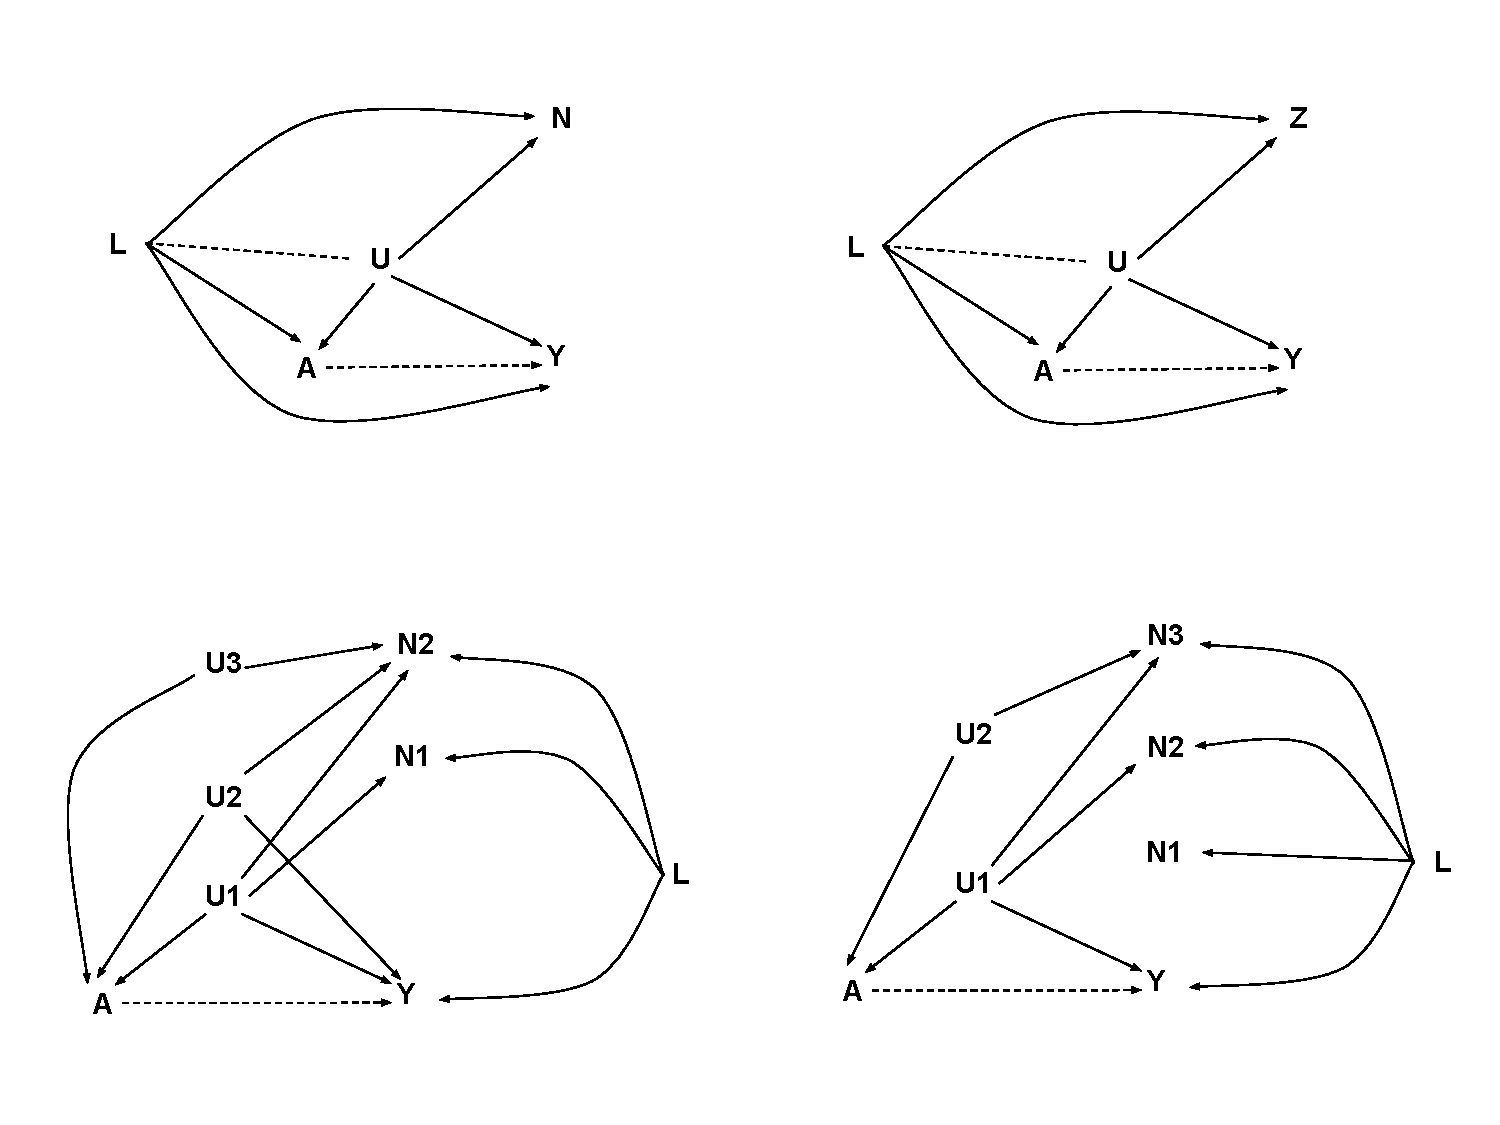
\includegraphics[trim={0 1cm 18cm 10cm}, clip, width=0.4\textwidth]{figures/dags.pdf}
    \caption[Causal DAG of two non-ideal NCOs $N1, N2$ for bias detection/correction of the effect of treatment $A$ on outcome $Y$.]{Causal DAG of two non-ideal NCOs $N1, N2$ for bias detection/correction of the effect of treatment $A$ on outcome $Y$, with unmeasured confounders $U1, U2, U3$. Observed confounders $L$ that cause $A, Y, N1, N2$ and may relate to $U1, U2, U3$ are not showed.}
    \label{fig:nco-nonideal-dag}
\end{figure}

Assumption \ref{as:ucomparability} means that the common causes of $A$ and an ideal NCO $N$ are \textit{identical} to those of $A$ and $Y$ \cite{lipsitch2010negative}. Similary, it means that the common causes of an ideal NCE $Z$ and $Y$ are identical to those of $A$ and $Y$ \cite{lipsitch2010negative}. Figure~\ref{fig:nco-nco-dag} and Figure~\ref{fig:nco-nce-dag} shows the causal DAGs of ideal an NCO and ideal NCE. Based on Assumptions \ref{as:nco}, \ref{as:nce}, and \ref{as:ucomparability}, empirical associations between the treatment and the NCO (or the NCE and the outcome), after controlling for all other observed variables $L$, are evidence of unmeasured confounding. For a comprehensive review, see Shi et al. \cite{shi2020selective}

In addition to bias detection, recent negative control techniques focus on partial or full bias correction \cite{shi2020selective}. Each technique has a unique set of assumptions and limitations. The following techniques partially correct for bias if their assumptions hold. Flanders et al. (2017) proposed adjusting for a negative control exposure to reduce bias in the estimate of the ATE using regression analyses. It works with time-series data but assumes linear relationships between the outcome and unmeasured confounders \cite{flanders2017new}. Schuemie et al. proposed empirical calibration of p-value \cite{schuemie2016robust} and empirical calibration of confidence intervals \cite{schuemie2018empirical} using a set of negative controls. These calibration techniques aim to robustly control the Type I error rate and reduce the number of falsely-rejected null hypothesis of no causal effect in the presence of unmeasured confounding. They assume that the negative controls (and positive for confidence interval calibration) are to some level exchangeable with the outcome, and the bias is approximately Gaussian. The calibrated p-value and confidence interval help control the Type I error rate, but at the cost of a potentially vast increase in the Type II error rate \cite{gruber2016limitations}.

The following techniques can fully correct for bias if their assumptions hold. Tchetgen Tchetgen (2014) proposed a control outcome calibration technique to remove the systematic bias in the estimate of the ATT using an NCO. It requires rank preservation (i.e. a constant additive individual treatment effect) \cite{tchetgen2014control}. Sofer et al. (2016) proposed a generalization of difference-in-differences as a negative control outcome approach to detect and correct for bias in the ATT estimate. It requires monotonic associations between unmeasured confounders and the control outcomes as well as the outcome of interest \cite{sofer2016negative}. Recent techniques using a pair of NCO and NCE, called double negative controls, provide nonparametric identification of the ATE \cite{miao2018identifying, shi2020multiply}. For inference on the true treatment effect, they require that both categorical negative controls have as many levels as the categorical unmeasured confounders and that at least one of the working models for the NCO or the outcome is correct.

\subsection{Our contribution}

Most negative control techniques rely on only one NCO and/or one NCE \cite{tchetgen2014control, sofer2016negative, flanders2017new, miao2018identifying, shi2020multiply}, while it can be advantageous to consider multiple negative controls.
Most techniques for bias correction also require that the negative control is U-comparable to the treatment and outcome of interest (i.e. Assumption \ref{as:ucomparability}) \cite{tchetgen2014control, flanders2017new, miao2018identifying, shi2020multiply}.
However, in practice, such negative controls are likely rare to find \cite{lipsitch2010negative}.
If $A$ and $N$ are confounded by some, but not all, variables in set $U$, they might appear unassociated even though unmeasured confounding exists for $A$ and $Y$ (see $N1$ in Figure~\ref{fig:nco-nonideal-dag}) \cite{lipsitch2010negative}. If $A$ and $N$ have an unmeasured common cause not in set $U$, an empirical association between $A$ and $N$ may not prove unmeasured confounding exists for $A$ and $Y$ (see $N2$ in Figure~\ref{fig:nco-nonideal-dag}) \cite{lipsitch2010negative}. When there is uncertainty about the confounding structure, a set of negative controls can be chosen to detect bias across multiple domains of confounding.

Many epidemiological studies have successfully used multiple negative controls for sensitivity analysis. For example, Jackson et al. (2006) used several NCOs to detect unmeasured confounding bias in unexpectedly large estimated benefits of influenza vaccine on seniors. The NCOs were risk of influenza hospitalization before and after flu seasons, and hospitalization of outcomes not linked to influenza \cite{jackson2006evidence}. Dormuth et al (2009) used a set of negative controls related to health behavior to detect bias due to the healthy user effect among new users of statins \cite{dormuth2009statin}. In a similar example, Lousdal et al. (2020) used multiple negative controls in an observational study of mammography screening participants and non-participants to caution against unmeasured confounding. They used proxies for better health, including death from various causes other than breast cancer, as NCOs and proxies for healthier behaviors, including dental care participation, as an NCE \cite{lousdal2020negative}. However, the problem of how to correct bias and draw conclusions about the validity of causal estimates from studies with multiple negative controls remains open.

There are several challenges to be considered. Firstly, existing bias correction techniques are likely to provide different corrected causal estimates for different negative controls. It is then unclear how to aggregate or interpret these corrected estimates, especially if they have opposing signs. Secondly, the estimated bias from each negative control will likely have different sizes and precisions, for example, due to differing sample sizes or incidence rates, or because the unmeasured confounding is stronger for one negative control than for another. The estimates may even have opposing signs. For example, if gender were an unmeasured confounder, then it may be promotive of prostate cancer but protective against breast cancer. The precision, direction of each negative control estimate, and variability among estimates should be taken into consideration when drawing conclusions. Though empirical calibration of p-value and confidence interval partially address these two challenges, these methods have low power to detect non-null causal effects when some bias estimates have opposing signs or are null \cite{gruber2016limitations}. Thirdly, it is possible that unmeasured confounding induces bias too small to affect the conclusion of the study. In that case, the bias can be safely ignored \cite{hernan2010causal}. Therefore, it is important to quantify the expected magnitude of the \textit{net} bias from all unmeasured confounders \cite{hernan2010causal, gruber2016limitations}. Though empirical calibration of p-value and confidence interval model the distribution of the bias, their calibrated test statistics blend unmeasured confounding bias and sampling variance into a single metric \cite{gruber2016limitations}. It would be advantageous to estimate the magnitude of the bias separately from random error and to provide uncertainty quantification for this estimated magnitude.

Based on these considerations, we propose a Bayesian hierarchical model to estimate the magnitude of the net unmeasured confounding bias, separately from its existence, its direction, and the random error. We view this partial bias correction approach as having the following advantages. Firstly, it infers a posterior distribution of the magnitude of the bias from multiple negative control estimates, providing uncertainty quantification for the estimated magnitude. Secondly, because the negative control estimates are residual biases after all other necessary adjustments, e.g. measured confounders, weighting, matching, censoring, etc., have been made, our proposed model can work with any complex study designs and any causal estimand that satisfies its modeling assumptions.
Thirdly, the proposed model can work with non-ideal NCOs, such as those in Figure~\ref{fig:nco-nonideal-dag}, and have assumptions less restrictive than the U-comparability, rank-preservation, and monotonicity assumptions of existing techniques. Though it shares many assumptions with empirical p-value calibration \cite{schuemie2016robust}, its ability to decompose the bias into its existence, direction, and magnitude makes it more suitable to model bias estimates from non-ideal negative controls.
Finally, the posterior of the magnitude of the bias enables the construction of a principled decision rule for whether to proceed with the study, in situations where prior information about the effect size may be available. Our proposed decision rule can guide researchers in refining their study design to a stage where the remaining bias may be considered negligible. We will focus solely on negative control outcomes below, though we believe extensions to negative control exposures will be similar.

\section{Methods}
\label{sec:nco_method}

\subsection{Setup}

We consider the application of NCOs to assess systemic bias due to unmeasured confounding in an observational study. In this section, we refer to bias with respect to a given study design as a non-zero log risk ratio or risk difference for an outcome with a null effect, even after controlling for all observed confounding factors. A study design for our purposes also includes the proposed model of the association between the treatment and outcome. Analyses of multiple NCOs are performed and result in a set of bias estimates and their corresponding standard errors.

\subsection{Assumptions}

Our method relies on the following assumptions:

\begin{assumption}
    Consistency \cite{naimi2023defining}, positivity \cite{naimi2023defining}, no interference \cite{naimi2023defining}, and conditional exchangeability (Assumption~\ref{as:conditional-exchangeability}) given all common causes $(L, U)$ of $A$ and $Y$.
\end{assumption}

\noindent \textbf{Assumption~\ref{as:nco}.} \textit{(Negative control outcomes)} $N^a = N \text{ and } N \perp A | U, L$ for all $a$.

\begin{assumption}
    The observed biases, for the NCOs and the outcome of interest, in terms of log risk ratio or risk difference, are approximately Gaussian, centered at the true biases, with standard deviation equaling the estimated standard error.
\end{assumption}

\begin{assumption}
    The true biases, for the NCOs and the outcome of interest, are drawn from a common distribution whose parameters can be estimated.
\end{assumption}

In this chapter, we model this common distribution with a mixture of distributions to decompose the existence, direction, and magnitude of the biases. We recommend picking a heterogeneous set of NCOs for this assumption to hold. Below, we will define a Bayesian hierarchical model for the magnitude of the confounding bias.

\subsection{Model details}

% \tikzstyle{VertexStyle} = [shape            = ellipse,
%                           minimum width    = 3ex,%
%                           draw]

% \tikzstyle{EdgeStyle}   = [->,>=stealth']

% \begin{tikzpicture}[->,>=stealth',auto,node distance=3cm,
%   thick,main node/.style={circle,draw,font=\sffamily\Large\bfseries},scale=.1]
% \node[main node] (1) {U};
% \node[main node] (2) [right of=1] {N};
% \node[main node] (3) [below of=1] {X};
% \node[main node] (4) [left of=1] {A};
% \node[main node] (5) [right of=3] {Y};
% \path[every node/.style={font=\sffamily\small}]
% (1) edge node {} (2)
% (1) edge node {} (3)
% (1) edge node {} (4)
% (1) edge node {} (5)
% (3) edge node {} (4)
% (3) edge node {} (2)
% (3) edge node {} (1)
% (3) edge node {} (5)
% (4) edge node {} (5)
% \end{tikzpicture}


The following model is for a binary treatment, binary outcome, and $I$ binary NCOs. Let $\widehat{S_{i}}$ be the bias estimates in terms of log risk ratio or risk difference for NCO $i=1,...,I$ under a binary treatment $A$, and $\widehat{\Sigma}$ be the bootstrap-estimated covariance of the random error in the bias estimates. We assume that the bias estimates are normally distributed around the true biases, and the estimated covariance adequately captures variation in the estimates due to random error:

\begin{align}
(\widehat{S}_{1},...,\widehat{S}_{I})^T &\sim N((S_{1}, . . . , S_{I})^T, \widehat{\Sigma} )
\end{align}

We also assume that the true biases are i.i.d. samples from a common bias distribution parametrized by a mixture of Gaussians and a point mass $P_0$ at zero:

\begin{align}
    S_{i} &\sim \delta_i P_0 + (1-\delta_i) (2M_i - 1) N(\mu, \sigma^2)
\end{align}

Parameter $\delta_i$ is an indicator for whether the $i$th bias belongs to the point mass or the Gaussian components. It models the existence of the $i$th bias, since it is possible for the overall bias for NCO $i$ to be null, for example when there are multiple sources of opposing bias. Parameter $M_i$ is an indicator for whether the bias belongs to the Gaussian component with a positive or a negative expectation. It models the direction of the bias. The motivation for this bimodal form is the following. Suppose that we have a single unmeasured confounding variable such as gender, then this variable may be promotive of prostate cancer but protective of breast cancer. The two Gaussian modes share the same variance $\sigma^2$ and an absolute value of the expectation $\mu$. These parameters characterize the magnitude of the bias. We place hierarchical priors on $\mu$ and $\sigma^2$:

\begin{align}
    \mu &\sim |N(\nu, \tau^2)|\\
    \sigma^2 &\sim |Cauchy(s_0)|
\end{align}

The reason for forcing $\mu$ to be nonnegative is to prevent identifiability issues due to the form of (2). Because the number of available NCOs is typically small, we can use a weakly informative half-Cauchy prior for $\sigma^2$ as suggested by \cite{gelman2006prior}, and recommend that scale $s_0$ be chosen based on the data application to construct an informative prior when possible. We also place priors on the bias existence and bias direction parameters:

\begin{align}
    \delta_i &\sim Bern(\phi_\delta)\\
    M_i &\sim Bern(\phi_M)\\
    \phi_M &\sim Beta(u_0, v_0) \\
    \phi_\delta &\sim Beta(r_0, s_0)
\end{align}

When the treatment groups are balanced and there is no confounding bias, $\phi_\delta$ will ideally be 1, and $\delta_i$ will be 1 for all $i$. Parameter $\phi_\delta$ gives the posterior predictive probability that the bias of a new outcome is null. Inference on $\{M_i\}_i^I, \phi_M$ is not of interest for our model. They exist to prevent biases of opposing signs from pulling the magnitude of the bias toward zero or inflating the magnitude's variance. When $u_0=v_0=1$ or $r_0=s_0=1$, these priors simplify to a uniform distribution that can be used as an uninformative prior. For an uninformative prior, we can set $\nu=0$ and $\tau^2=1^2$, though we recommend setting informative priors when possible.

We can extend this model to treatment with multiple treatment groups. A comparison of two treatment groups will be referred to as a treatment setting. Additional priors on $\nu$ and $\tau^2$ can also be specified to allow some sharing of information across the settings.

\subsection{Expected bias magnitude conditional on outcomes prevalence}

We observe that, on the risk difference scale, the estimated bias and its standard error tend to be greater when the NCO's prevalence---the average probability of observing the outcome in the population---is closer to 0.5, and smaller when it's closer to 0 or 1. On the log risk ratio scale, we also observe correlations between an NCO's prevalence and its bias' magnitude and variance. Figure~\ref{fig:nco-demo} shows log risk ratios and risk differences of simulated NCOs with identical associations to U but with different prevalence rates.

\begin{figure}[H]
    \centering
    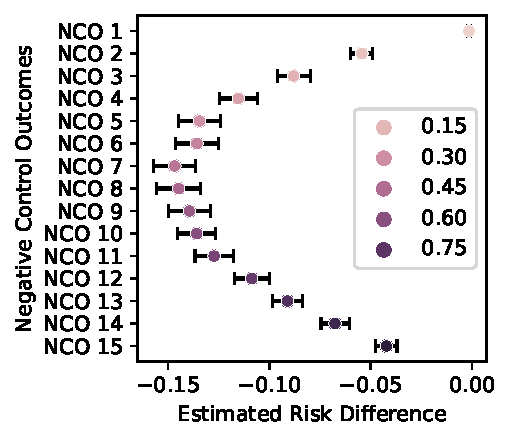
\includegraphics[width=0.45\textwidth]{figures/demo-rd.pdf}
    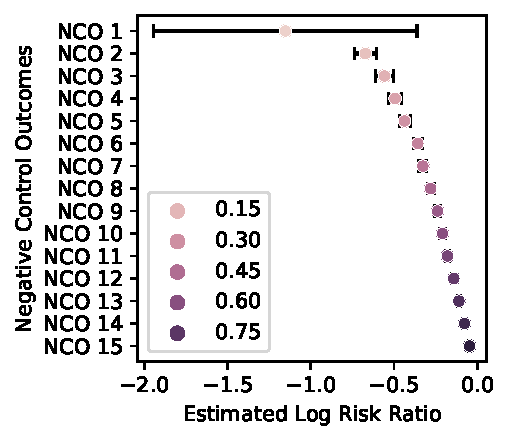
\includegraphics[width=0.45\textwidth]{figures/demo-lrr.pdf}
    \caption[Log risk ratios and risk difference of simulated NCOs with different outcome prevalence rates.]{Log risk ratios and risk difference of simulated NCOs with identical associations to unmeasured confounder $U$ but with different outcome prevalence rates.}
    \label{fig:nco-demo}
\end{figure}

As a result, we want to model $\mu$ and $\sigma^2$ as smooth functions of the outcome prevalence $x_i$. Therefore, we replace equation (3.3):

\begin{align}
    S_{i} &\sim \delta_i P_0 + (1-\delta_i) (2M_i - 1) N(\mu(x_i), \sigma^2(x_i))
\end{align}

One option is to fit a linear regression of polynomials of the prevalence. Here, we present another option to learn the functions by placing Gaussian process priors on the function $\mu(.)$ and $\sigma^2(.)$, replacing equations (3.4) and (3.5) with:

\begin{align}
    \mu &\sim |GP(f_1, c_\mu)| \\
    log(\sigma^2) &\sim GP(f_2, c_{\sigma^2})
\end{align}

\noindent where $f$ is a mean function and $c_\mu, c_{\sigma^2}$ is a covariance kernel. We choose to use the Gaussian kernel to model a smooth function $\mu$ and $\sigma^2$:

\begin{align}
    c_\mu(x_l, x_h) &= d_1 e^{- \frac{(x_l-x_h)^2}{2 \kappa_1^2}} \\
    c_{\sigma^2}(x_l, x_h) &= d_2 e^{- \frac{(x_l-x_h)^2}{2 \kappa_2^2}}
\end{align}

\noindent where $d_1, d_2$ are amplitude parameters and $\kappa_1, \kappa_2$ are length scales, which determine the wiggliness of the functions. We place informative priors on the length scales so that they are between 0 and 1 with 99\% probability, because input $x$ (outcome prevalence) ranges from 0 to 1. We recommend setting informative priors for $d_1 \sim |N(0, s_1)|$, $d_2 \sim |Normal(0, s_2)|$ by choosing $s_1, s_2$ based on the data. We set the mean function $f_1 = f_2 = 0$.

To predict the magnitude of the bias of a new outcome with proportion $x^\ast$, we use the property that $\mu(x_1),...,\mu(x_I), \mu(x^\ast)$ are jointly normal:

\begin{align}
    \begin{bmatrix}
    \mu \\
    \mu(x^\ast)
\end{bmatrix} &\sim |N(\boldsymbol{0},
\begin{bmatrix}
K & K^\ast\\
K^{\ast T} & c(x^\ast, x^\ast)
\end{bmatrix}
)|
\end{align}

where $K^\ast$ is the covariance between observed $\mu$ and new $\mu(x^\ast)$. Using the conditional normal formula, we can get a posterior predictive for $\mu(x^\ast)$:

\begin{align}
    p(\mu(x^\ast) | \mu) &\sim |N(A, V)| \\
    A &= K^{\ast T} K^{-1} \mu \\
    V &= c(x^\ast, x^\ast) - K^{\ast T} K^{-1} K^\ast
\end{align}

\subsection{Posterior computation}

We use PyMC for inference using Hamiltonian Monte Carlo.

\subsection{Decision rule}

We propose the construction of a decision rule based on a bias magnitude threshold parameter and a probability bound parameter. The probability bound parameter specifies how certain we want to be that the bias in the treatment-outcome association is less than the bias magnitude threshold parameter. For example, we might create an a priori decision rule stating that if the magnitude of the bias in terms of risk difference is less than 0.1 with at least 95\% probability, we will proceed with the study. In situations where they are available, the bias magnitude threshold parameter can be selected based on previous results. For example, if a previous study has shown an effect size difference of 0.3 between two populations that are comparable to those in the new study of interest, then a bias of 0.1 might be considered acceptable. If the estimated probability is less than the pre-specified probability bound parameter, the study may be abandoned since the results would potentially be invalid.

Procedurally, we specify a priori a decision rule that if the magnitude of the bias is less than $\theta$ with at least $\rho$\% probability, we will proceed with the study. Here, $\theta$ is the bias magnitude threshold parameter, and $\rho$ is the probability bound parameter, chosen based on domain expert knowledge.
% (Alternatively, a negative control study can be done after the study of interest, then the decision rule determines if we should consider the effect estimate of interest to be invalid or not.)
Using the posterior predictive distribution of the magnitude of the bias for a new outcome $p(S_{I+1}|\widehat{S}_{1},...,\widehat{S}_{I})$, we want to calculate $\pi=Pr(S_{I+1} < \theta | \widehat{S}_{1},...,\widehat{S}_{I})$---the posterior probability that the magnitude is less than $\theta$. If $\pi \geq \rho$, we may proceed with the study of interest.

We can approximate $\pi$ using Monte Carlo samples. Fixing $M_{I+1}=1$ or predicting $M_{I+1}$ using a signed causal diagram as discussed in \cite{hernan2010causal} (since we are mostly interested in the magnitude), for each $t \in {1, ..., T}$:
\begin{enumerate}
    \item sample $\delta_{I+1}^{(t)} \sim Bern(\phi_\delta^{(t)})$
    \item sample $S_{I+1}^{(t)} \sim  \delta_{I+1}^{(t)} P_0 + (1-\delta_{I+1}^{(t)})(2M_{I+1} - 1)N(\mu^{(t)}, \sigma^{2(t)})$
    \item compute $\pi^{(t)} = \mathbbm{1}(S_{I+1}^{(t)} < \theta)$
\end{enumerate}

where $T$ is the number of MCMC iterations; $\phi_\delta^{(t)}, \mu^{(t)}, \sigma^{2(t)}$ are posterior samples from the $t$th MCMC iteration. Finally, compute $\pi \approx \hat{\pi} = \frac{\sum_t \pi^{(t)}}{T}$.

\section{Simulations}
\label{sec:nco_sim}

\subsection{Similar outcome prevalence rates}

Data for $n=1,...,N$ where $N=10000$ subjects were generated according to the following scheme: the unobserved confounder of the treatment and outcome $U_n \sim N(0, 1)$, the treatment assignment $\text{logit}[P(A_n=1|U)] = 0.5 U_n$, the collection of $I$ negative control outcomes $\text{logit}[P(N_{i,n}=1|U)] = \alpha_{i} U_n$, and the relationships between $U$ and $N_i$ as $\alpha_{i} \sim 0.3P_0 + 0.2 Unif(0.5, 0.75) + 0.5 Unif(-0.75, -0.5)$ for $n=1,...,N; i=1,...,I$, where $P_0$ is a point mass at 0.
The outcome prevalance rates of all NCOs were around 0.5.
This scheme is similar to the simulations used in \citep{gruber2016limitations}.
Since there are no observed confounders, the bias in terms of the log risk ratio for NCO $i$ was estimated with $\widehat{S}_{i} = log(\overline{N_{i,1}}) - log(\overline{N_{i,0}})$, where $\overline{N_{i,a}} = \frac{\sum_n^{N} N_{i,n} \mathbbm{1}(A_n=a)}{\sum_n^{N} \mathbbm{1}(A_n=a)}$.
We use the mean model described in subsection 3.2.3 and the GP model described in subsection 3.2.4 to infer the posterior predictive distribution for the bias magnitude of the NCOs for a set of observed collection sizes of $I \in {5, 15, 30, 50}$.
We repeated the simulations 100 times.

\begin{figure}[H]
\centering
\begin{subfigure}{.45\textwidth}
	\centering
	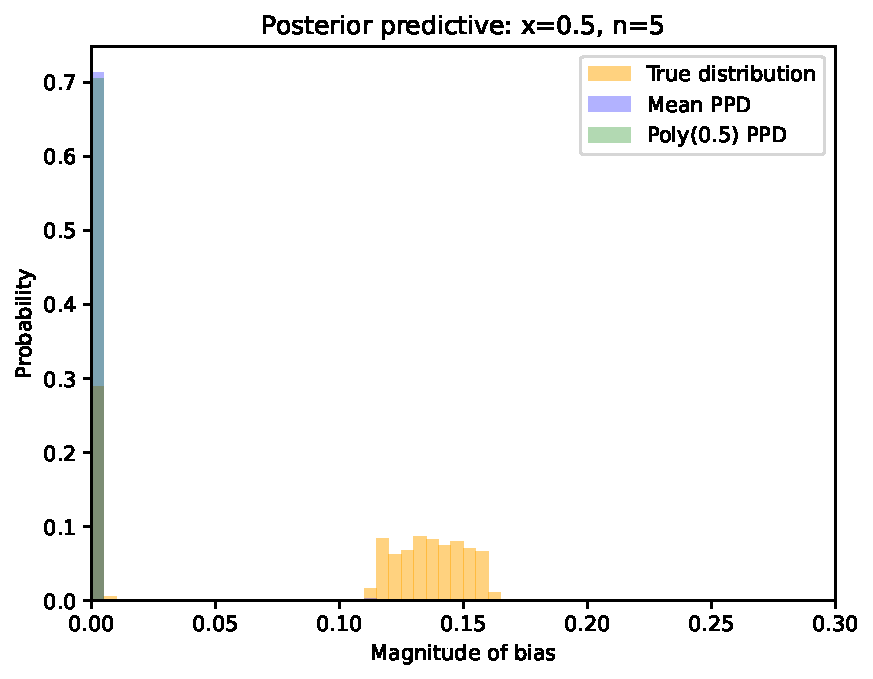
\includegraphics[width=0.9\textwidth]{figures/one-ppd-lrr-bias-5.pdf}
	\caption{I=5}
\end{subfigure}%
\begin{subfigure}{.45\textwidth}
	\centering
	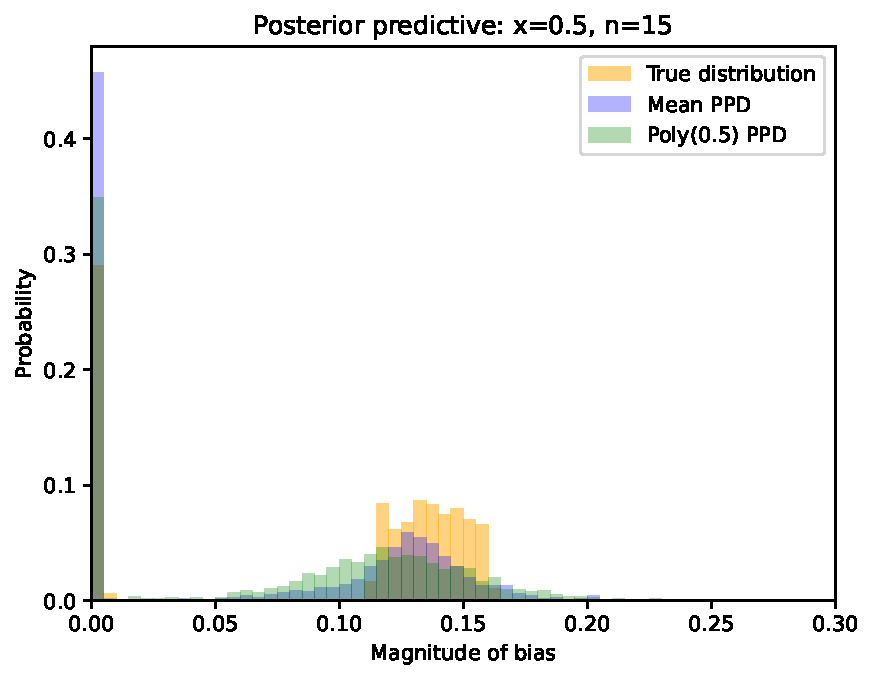
\includegraphics[width=0.9\textwidth]{figures/one-ppd-lrr-bias-15.pdf}
	\caption{I=15}
\end{subfigure}
\begin{subfigure}{.45\textwidth}
	\centering
	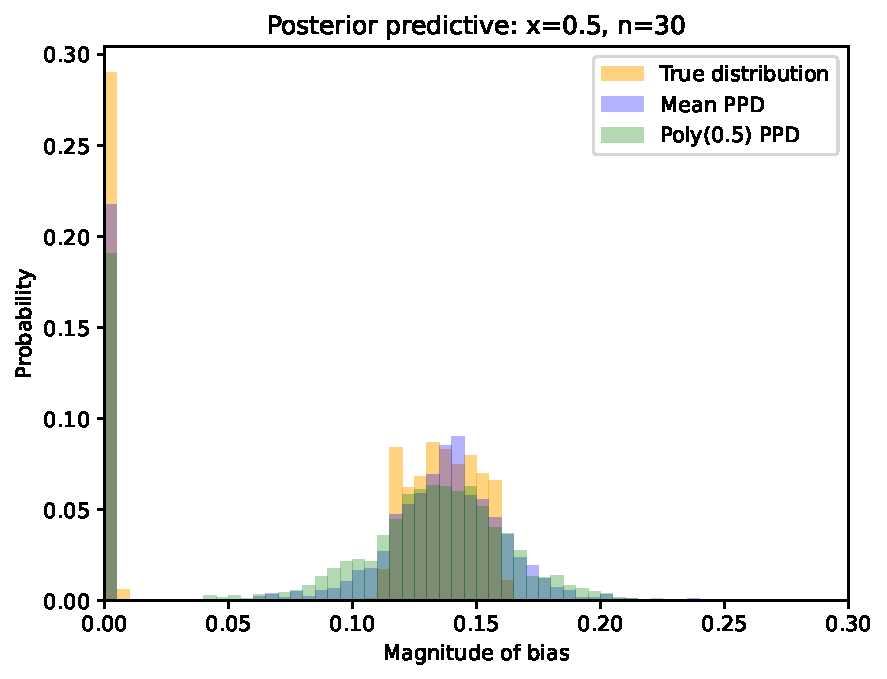
\includegraphics[width=0.9\textwidth]{figures/one-ppd-lrr-bias-30.pdf}
	\caption{I=30}
\end{subfigure}%
\begin{subfigure}{.45\textwidth}
	\centering
	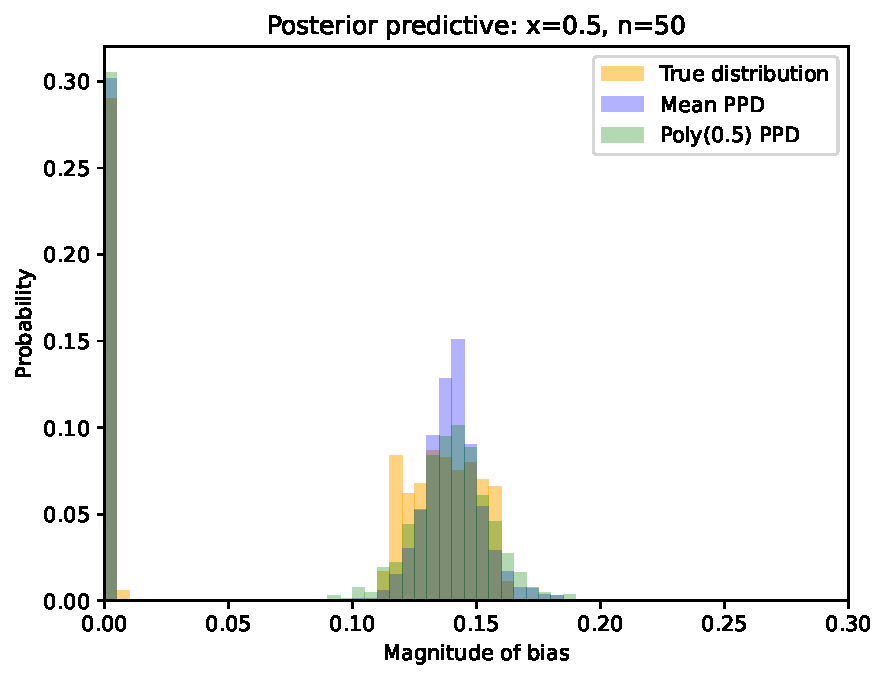
\includegraphics[width=0.9\textwidth]{figures/one-ppd-lrr-bias-50.pdf}
	\caption{I=50}
\end{subfigure}
\caption{Posterior predictive distributions using Mean and Polynomial model and varying number of observed NCOs. In yellow is the true distribution of bias for NCOs generated from schema in the simulation. As I increases, the posterior predictives become a better approximation of the true distribution of the bias.}
\end{figure}

For each simulation trial, we calculate two summary metrics: Wesserstain distance between true distribution and the posterior predictive distribution, and Absolute Percentage Difference (APD) between the 95th percentile of the true distribution and that of the posterior predictive distribution that is calculated as $(|\hat{q}-q|/q)100$\%. The table below mean and standard deviation in parenthesis of each metrics over 100 trials.

\begin{center}
\begin{tabular}{ |c|c|c|c| } 
\hline
Number of observed NCOs & Model & Wesserstain distance & APD from true 95th percentile\\ 
\hline
5 & Mean & 0.260 (0.193) & 818\% (672.6\%) \\
15 & Mean & 0.021 (0.011) & 16.6\% (15.0\%) \\
30 & Mean & 0.014 (0.007) & 6.1\% (4.8\%)\\
50 & Mean & \textbf{0.011} (0.006) & \textbf{5.1\%} (4.0\%)\\
5 & GP(0.5) & 1.146 (2.167) & 3371\% (6900\%)\\
15 & GP(0.5) & 0.030 (0.015) & 38.6\% (28.0\%)\\
30 & GP(0.5) & 0.015 (0.007) & 8.0\% (5.6\%)\\
50 & GP(0.5) & 0.012 (0.006) & 6.5\% (4.7\%)\\
\hline
\end{tabular}
\end{center}

\subsection{Differing outcome prevalence rates}

Now we consider a simulation setting with two sources of confounding and a set of NCOs that include 1) NCOs that have the same confounding structure as $A$ and $Y$; 2) NCOs that are caused by some, but not all, common causes of $A$ and $Y$; and 3) NCOs that are caused by a variable not a common cause of $A$ and $Y$. Data for $10000$ subjects were generated according to the following scheme:

\begin{align*}
    U_1 &\sim N(0, 1), \quad U_2 \sim N(0, 1)\\
    \text{logit}[P(A=1|U_1, U_2)] &= 0.3 U_1 + 0.4 U_2\\
    \text{logit}[P(N_{i}=1|U_1, U_2)] &= \nu_i + \alpha_{1,i} U_1 + \alpha_{2,i} U_2 \\
    \text{logit}[P(Y_l=1|A, U_1, U_2)] &= \nu^{(Y)} + \alpha^{(Y)}_{1,l} U_1 + \alpha^{(Y)}_{2, l}U_2 + \beta A\\
    \alpha_{j,i} &\sim 0.3P_0 + 0.49 Unif(0.5, 1) + 0.21 Unif(-1, -0.5)\\
    \alpha^{(Y)}_{j,l} &\sim 0.3P_0 + 0.49 Unif(0.5, 1) + 0.21 Unif(-1, -0.5)
\end{align*}

\noindent for $i=1,..., I; l=1,...,1000; j=1,2$, and NCO estimates in terms of log risk ratios are calculated as described in the last simulation. We set $\nu_i = logit(0.02 + (i - 1)\frac{0.9-0.02}{I})$ so that the outcome proportions of NCOs vary from $2\%$ to $90\%$. This will demonstrate the utility of having a flexible mean and variance function that accounts for outcome prevalence. We evaluate the ability of the mean model in subsection 3.2.3 and the Gaussian process model in subsection 3.2.4 to construct good posterior predictive distribution for bias in terms of log risk ratio conditional on the prevalence of unseen outcomes. We use our proposed decision rule to evaluate these simulations. A priori, we say that the bias is negligible if the bias in terms of log risk ratio is less than a bias threshold $\theta = 0.095$ with 95$\%$ probability. In each of 100 simulation replicates, we calculate $\pi$, the probability that true bias is less than $\theta$, using 1000 pairs of $A-Y$. We also estimate $\hat{\pi}_{mean}$ and $\hat{\pi}_{gp}$ from the posterior predictive of the models as outlined in subsection 3.2.6. We repeat everything for different $I=5, 15, 30, 50$ and different outcome prevalence rates $\nu^{(Y)} = logit(0.5), logit(0.05), logit(0.85)$.

\todo{Show results}

\section{Analysis of real data}
\subsection{Data description}
\todo{Write}
\subsection{Results}

\section{Discussion}

%%% Local Variables:
%%% mode: latex
%%% TeX-master: "nco-bias-characterization.tex"
%%% End:


% Acknowledgements should go at the end, before appendices and references

\acks{We would like to acknowledge support for this project from Obi-Wan Kenobi of the Galactic Republic.}

% Manual newpage inserted to improve layout of sample file - not
% needed in general before appendices/bibliography.

\newpage

% Note: in this sample, the section number is hard-coded in. Following
% proper LaTeX conventions, it should properly be coded as a reference:

%In this appendix we prove the following theorem from
%Section~\ref{sec:textree-generalization}:

\vskip 0.2in
\bibliography{refs}

\appendix
\section*{Appendix A.}
\label{app:theorem}

In this appendix we prove the following theorem from
Section~6.2:

\ldots

\end{document}
